\section{Hubs}
An Ethernet hub or hub is a device for connecting multiple Ethernet devices together and making them act as a single network segment. It has multiple input/output (I/O) ports, in which a signal introduced at the input of any port appears at the output of every port except the original incoming. A hub works at the physical layer (layer 1) of the OSI model.
 A hub does not examine or manage any of the traffic that comes through it: any packet entering any port is rebroadcast on all other ports.
 It is barely aware of frames or packets and mostly operates on raw bits or symbols. Consequently, due to the larger collision domains, packet collisions are more frequent in networks connected using hubs than in networks connected using more sophisticated devices.
 Hubs are classified as physical layer devices in the OSI model. At the physical layer, hubs support little in the way of sophisticated networking. Hubs do not read any of the data passing through them and are not aware of their source or destination addressing. A hub simply receives incoming Ethernet frames, regenerates the electrical signal on the bit (more precisely the symbol) level, and broadcasts these symbols out to all other devices on the network.
 \begin{figure}[htbp]
\begin{center}
	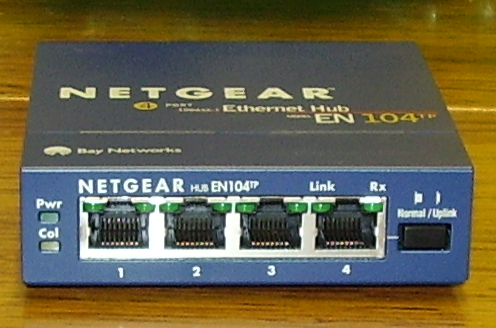
\includegraphics[width=5cm]{./Networking/ntwhardware/hub.jpg}
\caption{Network Hub}
\label{default}
\end{center}
\end{figure}
